\documentclass[12pt,letter]{article}


\usepackage{nicefrac,amsmath}
\usepackage[english]{babel}
\usepackage{helvet}
\usepackage{enumerate}
\usepackage{parskip}
%\usepackage{apacite}
\usepackage[english]{babel}
\usepackage{booktabs}
\usepackage[top=1in, bottom=1in, left=1in, right=1in]{geometry}
\usepackage{graphicx}
\usepackage{subfigure}
\usepackage{url}
\usepackage{hyperref}
\usepackage{physics}
\usepackage{cancel}
\usepackage{gensymb}
\usepackage{bbm}
\usepackage{dsfont}
\usepackage{mathtools}
\usepackage{appendix}
\usepackage{etoolbox}

\usepackage{amsfonts}

% Inserts \clearpage before \begin{appendices}
\BeforeBeginEnvironment{appendices}{\clearpage}

\usepackage{algpseudocode}
\usepackage{algorithm}


\usepackage[usenames,dvipsnames]{color}
 \usepackage{listings}
 \definecolor{Brown}{cmyk}{0,0.81,1,0.60}
 \definecolor{OliveGreen}{cmyk}{0.64,0,0.95,0.40}
 \definecolor{CadetBlue}{cmyk}{0.62,0.57,0.23,0}



 \lstset{language=C,%basicstyle=\normalsize,
 keywordstyle=\ttfamily\color{OliveGreen}\bfseries,
 identifierstyle=\ttfamily\color{CadetBlue}\bfseries, 
 commentstyle=\color{Brown}\ttfamily,
 stringstyle=\ttfamily\color{red},
 showstringspaces=false}


\newcommand{\argmax}[1]{\underset{#1}{\operatorname{arg}\,\operatorname{max}}\;}
\newcommand{\argmin}[1]{\underset{#1}{\operatorname{arg}\,\operatorname{min}}\;}


\newcommand{\R}{\mathbb{R}}

%\usepackage{cmbright}
\usepackage[T1]{fontenc}

\setlength{\parskip}{12pt} % 1ex plus 0.5ex minus 0.2ex}

%\renewcommand{\familydefault}{\sfdefault}

\setlength{\parindent}{0cm}
\renewcommand{\baselinestretch}{1.2}

\title{{\bf Geometric transformations in 2-D} }


\date{}
\begin{document}
\maketitle
\vspace{-1.0in}

%{\small 
%\tableofcontents
%%\listoffigures
%%\listofalgorithms
%}

%\newpage

\section{Overview}
In these notes, we introduce the topic of two-dimensional geometric
transformations. We begin with the definition of the basic single-valued
linear function, which we then upgrade to its two-dimensional
counterpart. The 2-D transformation usually consists of two separate
equations, each generating a component of the transformed vector by
combining (i.e., mixing) the components of the original input vector
with the parameters of the transformation. When these transformations
are linear, they can be written in matrix form which allows us to take
advantage of the tools of matrix algebra and linear algebra. By using
matrices to represent transformations, we can perform efficient
computations on large quantities of data as well as write formulations
that are both elegant and concise.

%% New section
\section{One-dimensional linear transformations}

The function $f: \mathbb{R} \rightarrow \mathbb{R}$ such that:
\begin{align}
	f(x) = ax,
		\label{linear1D}
\end{align}
with $a \in \R$ is a simple case of a 1-D linear transformation. It
maps (i.e., transforms) the value $x$ onto a new value $ax$. For example, $f\left(x\right) = 3x$ maps an input value $x$ into its triple.

\section{2-D (Linear) Geometric
Transformations}

The 2-D extension of the function in Equation \(\ref{linear1D}\)
transforms two-dimensional vectors \({\bf x} = (x,y)^\mathsf{T}\) onto
two-dimensional vectors. In this case, we write
\(f: \mathbb{R}^2 \rightarrow \mathbb{R}^2\) such that:
\begin{align}
		x^\prime = f_1\left(x,y\right) = a_1 x + a_2 y, \notag \\
		y^\prime = f_2\left(x,y\right) = a_3 x + a_4 y.
		\label{2Dlinear}
\end{align}
In the 2-D case, the linear transformation consists of two separate
equations, each resulting in one component (or coordinate) of the
transformed vector. Equation \(\ref{2Dlinear}\) can be written in matrix
form as:
\begin{align}
		\begin{bmatrix}
		x^\prime \\
		y^\prime
	\end{bmatrix}	
 	=
	\begin{bmatrix}
		a_1 & a_2 \\
		a_3 & a_4
	\end{bmatrix}
	\begin{bmatrix}
		x \\
		y
	\end{bmatrix},	
\end{align}
or, in short:
\begin{align}
	{\bf x}^\prime = A{\bf x}.
	\label{linearND}
\end{align}
Note that Equations \(\ref{linear1D}\) and \(\ref{linearND}\) have the
same overall form but the 2-D version maps vectors instead of numbers,
and the transformation is represented by a \(2\times2\) matrix:
\begin{align}
	A = 
	\begin{bmatrix}
		a_1 & a_2 \\
		a_3 & a_4
	\end{bmatrix}.
\end{align}
This matrix is called the {\em matrix of the linear transformation}.

\section{Some important 2-D geometric
transformations}

The matrix of some important linear geometric 2-D transformations are:

\paragraph{Scaling:}
\begin{align}
	S = 
	\begin{bmatrix}
		s_x & 0 \\
		0 & s_y
	\end{bmatrix}. 
\end{align}


\paragraph{Rotation:}

\begin{align}
	R = 
	\begin{bmatrix}
		\cos\theta & -\sin\theta \\
		\sin\theta &  \cos\theta 
	\end{bmatrix}.
\end{align}


\paragraph{Shearing:}

\begin{align}
	S_x = 
	\begin{bmatrix}
		1 & k \\
		0 &  1 
	\end{bmatrix} 
	\hspace{.2in}\text{and}\hspace{.2in}
	S_y = 
	\begin{bmatrix}
		1 & 0 \\
		k &  1 
	\end{bmatrix}, 
\end{align}
where \(S_x\) is a horizontal shear (i.e., parallel to the \(x\)-axis), and \(S_y\) is a vertical shear (i.e., parallel to the \(y\)-axis).

\section{Examples}
\label{examples}

\subsection{Transforming a single point} 
Consider the following scaling transformation matrix:
\begin{align}
	A = 
	\begin{bmatrix}
		2 & 0 \\
		0 & 3
	\end{bmatrix}, 
\end{align}
which we can use the matrix to transform the point \({\bf x} = (9, 6)^\mathsf{T}\) as follows:
\begin{align}
	{\bf x}^\prime &= A{\bf x}  \notag\\
	\begin{bmatrix}
		x^\prime \\
		y^\prime
	\end{bmatrix}	
 	&=
	\begin{bmatrix}
		2 & 0 \\
		0 & 3
	\end{bmatrix}
	\begin{bmatrix}
		9 \\
		6
	\end{bmatrix}	
 \notag\\
 	&=
	\begin{bmatrix}
		\left(2 \times 9\right) + \left(0   \times 6\right)\\
		  \left(0 \times 9\right) + \left(3 \times 6\right)
	\end{bmatrix} \notag\\
 	&=
	\begin{bmatrix}
		18\\
		18
	\end{bmatrix}.
	\label{scalingExample1}
\end{align}

\subsection{Transforming a shape (or polygon) given
by a set of vertices}

Equation \(\ref{scalingExample1}\) transformed a single 2-D point. To
transform a whole shape represented by a set of \(n\) 2-D vertices, we can transform each individual point of the shape (i.e., vertices) by repeatedly applying Equation \(\ref{scalingExample1}\). Alternatively, we 
can collect all vertices of the shape as columns of a matrix, and then
apply the transformation just as we did before for the single-point
case, i.e.:
\begin{align}
	X^\prime &= A\,X \\\notag\\
  \underbrace{\begin{bmatrix}    
  x_1^\prime & x_2^\prime & \hdots &x_n^\prime\\    
  y_1^\prime & y_2^\prime & \hdots &y_n^\prime  
  \end{bmatrix}}_{X^\prime}   	&=
	\underbrace{\begin{bmatrix}
		a_1 & a_2 \\
		a_3 & a_4
	\end{bmatrix}}_{A}\,
	\underbrace{\begin{bmatrix}
		x_1 & x_2 & \hdots &x_n\\
		y_1 & y_2 & \hdots &y_n
	\end{bmatrix}}_{X}.	
\end{align}
Here, matrix \(X^\prime\) is the transformed shape. Computationally, this approach is usually much faster than looping through all points to transform them individually. Also, using a matrix to represent the entire shape shortens the mathematical notation. 

For example, given a rectangle described by a set of four 2-D points,
\({\bf p}_i =
\left( x_i, y_i\right)^\mathsf{T}\), for \(i=1,..., 4\). We can store
these points in a single matrix, \(X\), as follows:

\begin{align} 
  X = 
  \begin{bmatrix}
      {\bf p}1 & {\bf p}2 & {\bf p}3 &{\bf p}4 
  \end{bmatrix} 
  = 
\begin{bmatrix} 
	 0 & 4 & 4 & 0\\
		0 & 0 & 2 & 2  
\end{bmatrix}   
\end{align}


We can then scale the entire shape by transforming it with the scale
transformation from Example 1 (Equation \(\ref{scalingExample1}\)) as
follows:
\begin{align}
 X^\prime
 	&=
	\begin{bmatrix}
		2 & 0 \\
		0 & 3
	\end{bmatrix}
	 \begin{bmatrix}      
	 0 & 4 & 4 & 0\\ 
	 0 & 0 & 2 & 2  
	 \end{bmatrix} 
 	=
	\begin{bmatrix}
	 0 & 8 & 8 & 0\\    
	 0 & 0 & 6 & 6  
	\end{bmatrix}. 
	\label{scalingExample3}
\end{align}
Figure \ref{fig_plot} shows the original and transformed shapes. 

\begin{figure}[ht]
	\begin{center}
		{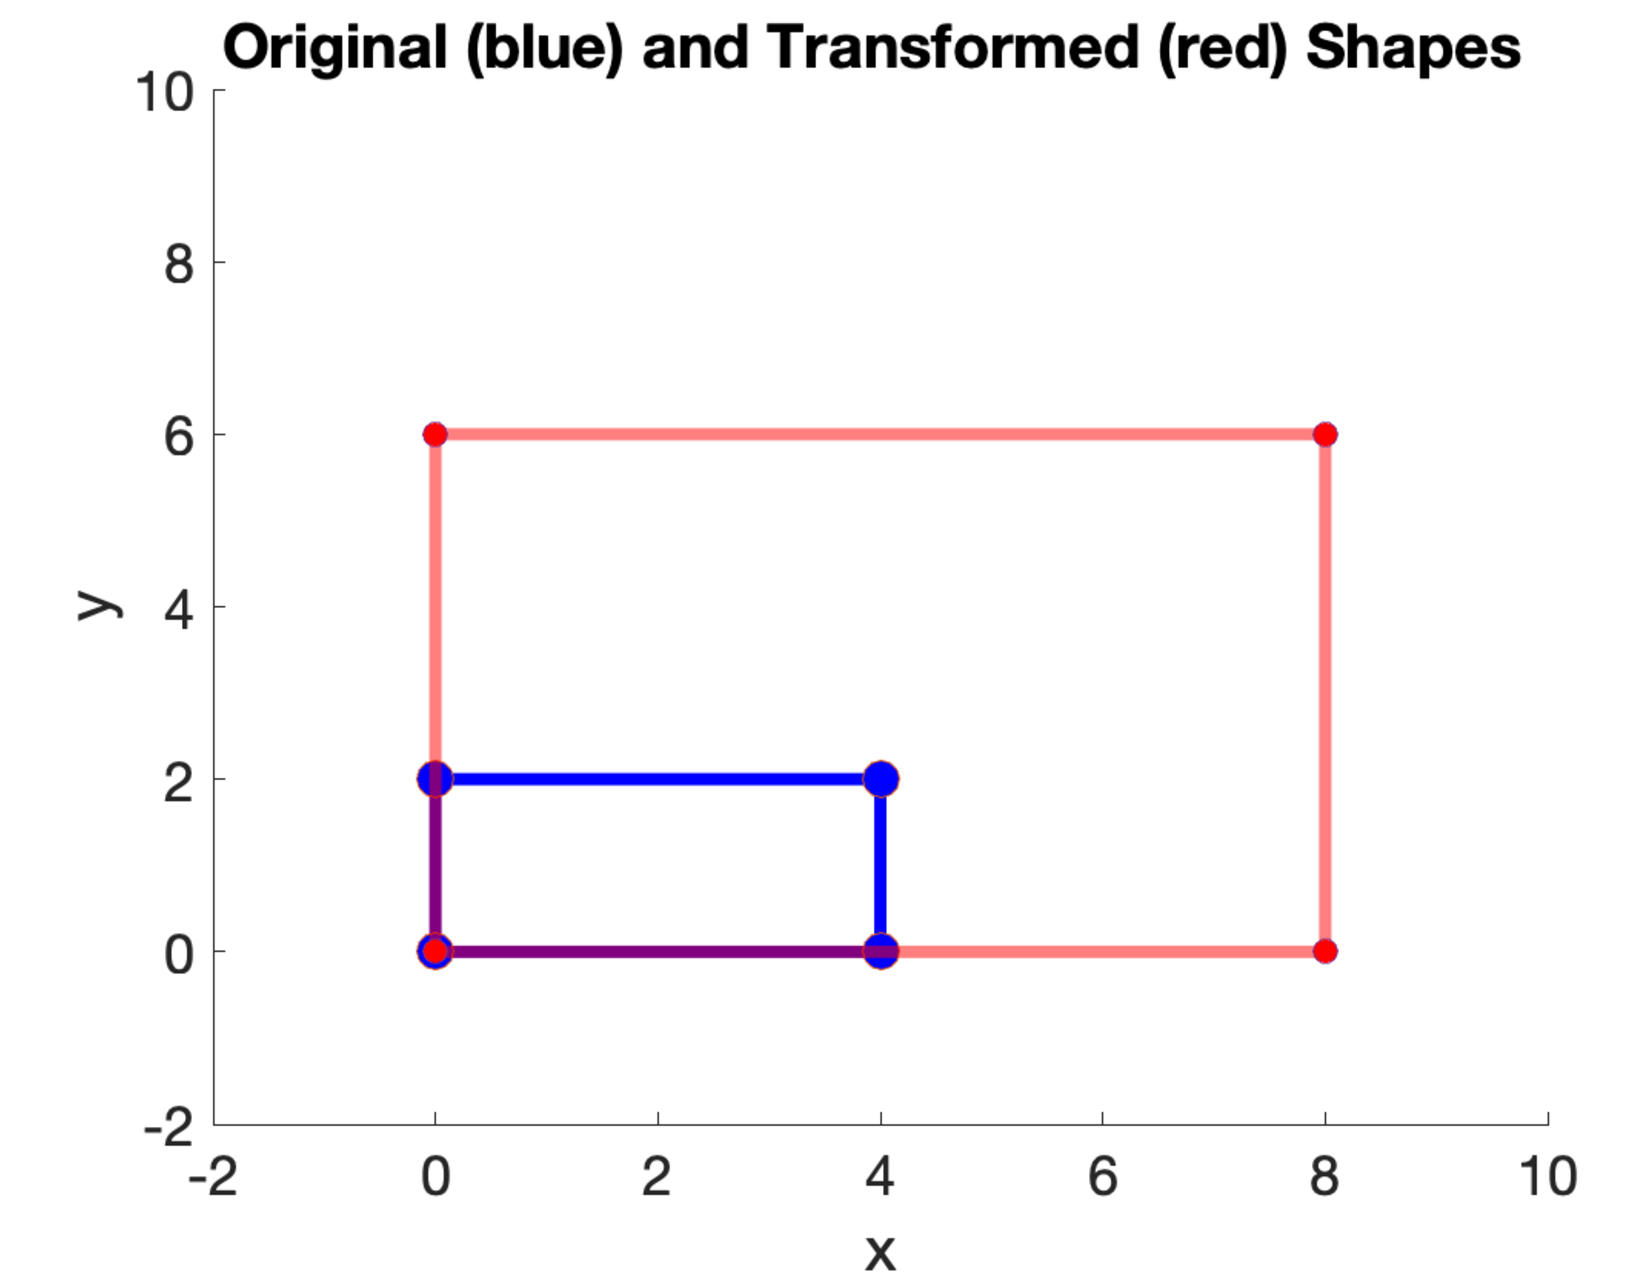
\includegraphics[width=.70\textwidth]{figs/plot}}
	\end{center}
	\caption{Scaling a rectangle. }
	\label{fig_plot}
\end{figure}



%% References 
\bibliographystyle{unsrt} 
\bibliography{refs}

\end{document}
% end of file template.tex




